% =====================================================================
%  Proyecto Final Integrador - Análisis de Algoritmos (SIST0175)
%  Grupo 6 - Avance (sesión 2): C1, C2 y C3
%  Compila con XeLaTeX o con pdfLaTeX (en Overleaf: Menu > Compiler).
% =====================================================================
\documentclass[11pt,letterpaper]{article}
\usepackage{iftex}
\ifXeTeX
  \usepackage{fontspec}
  \usepackage{polyglossia}
  \setmainlanguage{spanish}
  \gappto\captionsspanish{\renewcommand{\tablename}{Tabla}\renewcommand{\listtablename}{Índice de tablas}}
\else
  \usepackage[utf8]{inputenc}
  \usepackage[T1]{fontenc}
  \usepackage{lmodern}
  \usepackage[spanish,es-noshorthands,es-nodecimaldot,es-tabla]{babel}
\fi
\usepackage[margin=2.3cm]{geometry}
\usepackage{amsmath,amssymb,amsthm,mathtools}
\usepackage{graphicx,float,booktabs,array,tabularx,multirow}
\usepackage[table]{xcolor}
\usepackage{caption,subcaption}
\usepackage{algorithm}
\usepackage[noend]{algpseudocode}
\usepackage{tikz}
\usetikzlibrary{arrows.meta,positioning,fit,backgrounds,calc}
\usepackage{enumitem}
\usepackage{fancyhdr}
\usepackage{listings}
\definecolor{codfondo}{HTML}{F7F9FB}
\definecolor{codcoment}{HTML}{3B7D4F}
\definecolor{codcadena}{HTML}{A3452C}
\definecolor{codclave}{HTML}{1F5FA0}
\lstset{
  language=Python, basicstyle=\ttfamily\scriptsize, columns=fullflexible, keepspaces=true,
  backgroundcolor=\color{codfondo}, frame=single, rulecolor=\color{gris!40},
  numbers=left, numberstyle=\tiny\color{gris}, numbersep=6pt, xleftmargin=1.6em,
  breaklines=true, breakatwhitespace=false, postbreak=\mbox{\textcolor{gris}{$\hookrightarrow$}\space},
  keywordstyle=\color{codclave}\bfseries, commentstyle=\color{codcoment}\itshape,
  stringstyle=\color{codcadena}, showstringspaces=false, tabsize=4, upquote=true,
  extendedchars=true,
  literate={á}{{\'a}}1 {é}{{\'e}}1 {í}{{\'i}}1 {ó}{{\'o}}1 {ú}{{\'u}}1 {ñ}{{\~n}}1
           {Á}{{\'A}}1 {É}{{\'E}}1 {Í}{{\'I}}1 {Ó}{{\'O}}1 {Ú}{{\'U}}1 {Ñ}{{\~N}}1
           {¿}{{?`}}1 {¡}{{!`}}1 {²}{{\textsuperscript{2}}}1 {³}{{\textsuperscript{3}}}1
           {ĉ}{{$\hat{c}$}}1 {Θ}{{$\Theta$}}1 {Σ}{{$\Sigma$}}1 {φ}{{$\varphi$}}1
           {⌈}{{$\lceil$}}1 {⌉}{{$\rceil$}}1 {≤}{{$\le$}}1 {≥}{{$\ge$}}1 {→}{{$\to$}}1
}
\lstdefinestyle{salida}{language={}, numbers=none, xleftmargin=0pt, keywordstyle={}, commentstyle={}, stringstyle={}}
\newcommand{\codigo}[2]{\par\smallskip\noindent{\small\bfseries\texttt{\detokenize{#1}}}\enspace{\small\color{gris}#2}\lstinputlisting{codigo/#1}}
\usepackage[hidelinks]{hyperref}

\definecolor{azul}{HTML}{2A6FB0}
\definecolor{gris}{HTML}{5F6B76}
\definecolor{fondo}{HTML}{EEF3F8}
\captionsetup{font=small,labelfont=bf}
\setlist{itemsep=2pt,topsep=3pt}
\setlength{\parskip}{4pt}
\setlength{\parindent}{0pt}
\emergencystretch=3em
\tolerance=2000

\pagestyle{fancy}
\fancyhf{}
\lhead{\small\color{gris}Análisis de Algoritmos (SIST0175) -- Grupo 6}
\rhead{\small\color{gris}Avance: C1, C2 y C3}
\cfoot{\small\thepage}
\renewcommand{\headrulewidth}{0.3pt}

% Pseudocódigo en español
\floatname{algorithm}{Algoritmo}
\algrenewcommand\algorithmicwhile{\textbf{mientras}}
\algrenewcommand\algorithmicdo{\textbf{hacer}}
\algrenewcommand\algorithmicfor{\textbf{para}}
\algrenewcommand\algorithmicif{\textbf{si}}
\algrenewcommand\algorithmicthen{\textbf{entonces}}
\algrenewcommand\algorithmicelse{\textbf{si no}}
\algrenewcommand\algorithmicreturn{\textbf{devolver}}
\algrenewcommand\algorithmicfunction{\textbf{función}}
\algrenewcommand\algorithmicrequire{\textbf{Entrada:}}
\algrenewcommand\algorithmicensure{\textbf{Salida:}}
\algrenewcommand{\algorithmiccomment}[1]{\hfill{\color{gris}\(\triangleright\) #1}}

\theoremstyle{plain}
\newtheorem{teorema}{Teorema}
\newtheorem{lema}{Lema}
\theoremstyle{definition}
\newtheorem{definicion}{Definición}
\newcommand{\Th}{\Theta}
\newcommand{\Om}{\Omega}
\newcommand{\cajah}[1]{\par\smallskip\colorbox{fondo}{\parbox{\dimexpr\linewidth-2\fboxsep}{\small #1}}\par\smallskip}

\begin{document}

% ------------------------------------------------------------- PORTADA
\begin{titlepage}
\thispagestyle{empty}
\centering
{\large\textsc{Universidad Sergio Arboleda}\par}
\vspace{2mm}
{\normalsize Escuela de Ciencias Exactas e Ingeniería\par}
{\normalsize Programa de Ciencias de la Computación e Inteligencia Artificial\par}
\vspace{2.2cm}
{\large Análisis de Algoritmos (SIST0175)\par}
\vspace{6mm}
{\color{azul}\rule{0.7\linewidth}{0.8pt}\par}
\vspace{4mm}
{\LARGE\bfseries Proyecto Final Integrador\par}
\vspace{3mm}
{\Large Percepción y navegación de un vehículo autónomo urbano\par}
\vspace{3mm}
{\large Avance (sesión 2): componentes C1, C2 y C3\par}
{\color{azul}\rule{0.7\linewidth}{0.8pt}\par}
\vspace{2.2cm}
{\large\bfseries Grupo 6\par}
\vspace{3mm}
{\large Sebastián Páez Castañeda\par
Johan Sebastián Acuña\par
Santiago Felipe Fajardo\par}
\vspace{1.8cm}
{\normalsize Docente: Juan David Rodríguez Martínez\par}
\vfill
{\normalsize Bogotá D.C., noviembre de 2026\par}
\end{titlepage}

\tableofcontents
\vspace{6mm}
\cajah{\textbf{Contenido del entregable.} Este único PDF contiene los tres elementos solicitados:
\begin{enumerate}[leftmargin=1.5em,itemsep=0pt,topsep=2pt]
  \item \textbf{Código de C1, C2 y C3 con pruebas:} Anexo~\ref{anexo:codigo} (pág.~\pageref{anexo:codigo}),
  con el código fuente completo, sus pruebas \texttt{pytest} y la salida de su ejecución (23 pruebas aprobadas).
  \item \textbf{Análisis teórico de C1 a C3:} sección~\ref{sec:teoria} (pág.~\pageref{sec:teoria}).
  \item \textbf{Plan de experimentos con hipótesis:} sección~\ref{sec:plan} (pág.~\pageref{sec:plan}),
  junto con el generador de datos (sección 1 y Anexo~\ref{anexo:codigo}).
\end{enumerate}
Adelantamos además la validación empírica de C1--C3 (sección~\ref{sec:validacion}).}
\newpage
% ------------------------------------------------------------- 1. CASO
\section{Descripción del caso}

Un vehículo autónomo recorre una ciudad sintética de $1\,\text{km}\times 1\,\text{km}$. Sus sensores
producen una nube de puntos (LiDAR) que el sistema usa para tres tareas de este avance:
\begin{itemize}
  \item \textbf{C1 -- Distancia mínima entre obstáculos.} Los obstáculos detectados se proyectan al
  plano como $n$ puntos $(x,y)$. La distancia mínima entre ellos indica, por ejemplo, si el hueco
  más estrecho de la escena permite el paso del vehículo.
  \item \textbf{C2 -- Mapa de vóxeles.} La nube 3D se discretiza en cubos de lado $r$ (vóxeles).
  Solo se guardan los vóxeles ocupados, con su número de puntos, en una tabla hash dinámica.
  \item \textbf{C3 -- Cobertura de la trayectoria.} La trayectoria planeada es el segmento $[0,L]$;
  cada sensor (cámara, radar, unidad de borde) cubre un tramo $[a_i,b_i]$. Se busca el mínimo
  número de tramos que cubran todo $[0,L]$.
\end{itemize}

\textbf{Supuestos.} Coordenadas en metros como números de punto flotante; distancia euclidiana;
intervalos cerrados; datos sintéticos generados con semilla fija (\texttt{SEMILLA = 6}).

\textbf{Generador de datos} (\texttt{datos/generador.py}, NumPy \texttt{default\_rng(6)}):
\begin{itemize}
  \item \texttt{nube\_puntos\_2d(n, distribucion)}: \emph{uniforme} (caso esperado),
  \emph{agrupada} ($\sqrt n$ obstáculos con puntos gaussianos alrededor) y \emph{vertical}
  (todas las $x$ casi iguales: toda la nube cae en la franja central de C1).
  \item \texttt{escena\_urbana\_3d(P, L)}: puntos sobre el suelo, fachadas de cuatro edificios y
  postes; \texttt{claves\_distintas(n)}: $n$ claves de vóxel distintas para medir inserciones.
  \item \texttt{tramos\_sensado(n)}: $n$ tramos desordenados sobre $[0,n]$; una ``columna'' de
  $\approx n/10$ tramos solapados garantiza que exista cobertura.
  \texttt{tramos\_pequenos(n)}: instancias pequeñas (posiblemente infactibles) para fuerza bruta.
\end{itemize}

% ------------------------------------------------------------- 2. ARQUITECTURA
\section{Arquitectura}

\begin{figure}[H]
\centering
\begin{tikzpicture}[
  font=\small,
  caja/.style={draw=azul, rounded corners=3pt, fill=white, align=center, minimum width=3.3cm, minimum height=1.05cm, line width=0.7pt},
  futura/.style={caja, draw=gris, dashed, text=gris},
  dato/.style={draw=gris, fill=fondo, rounded corners=2pt, align=center, minimum width=3.0cm, minimum height=0.8cm},
  flecha/.style={-{Stealth[length=2.2mm]}, gris, line width=0.6pt},
  node distance=0.55cm and 0.9cm]
  \node[dato] (gen) {Generador\\ \footnotesize semilla 6};
  \node[dato, right=of gen, xshift=-0.3cm] (nube) {Nube LiDAR 3D};
  \node[dato, right=of nube] (tray) {Trayectoria $[0,L]$\\ y sensores};
  \node[dato, right=of tray, xshift=-0.3cm] (tel) {Telemetría\\ \footnotesize (marcas de tiempo)};

  \node[caja, below=1.0cm of nube, xshift=-2.2cm] (c1) {\textbf{C1} Par más cercano\\ \footnotesize D\&V, $\Th(n\log n)$};
  \node[caja, right=0.35cm of c1] (c2) {\textbf{C2} Mapa de vóxeles\\ \footnotesize tabla hash, $O(1)$ amort.};
  \node[caja, right=0.35cm of c2] (c3) {\textbf{C3} Cobertura mínima\\ \footnotesize voraz, $\Th(n\log n)$};

  \node[futura, below=0.9cm of c1] (c4) {\textbf{C4} Backtracking\\ \footnotesize parqueo / evasión};
  \node[futura, right=0.35cm of c4] (c5) {\textbf{C5} Árbol B+ en disco\\ \footnotesize telemetría por tiempo};
  \node[futura, right=0.35cm of c5] (c6) {\textbf{C6} Cobertura de vértices\\ \footnotesize 2-aproximación};

  \draw[flecha] (gen) -- (nube);
  \draw[flecha] (nube.south) -- ++(0,-0.35) -| (c1.north);
  \draw[flecha] (nube.south) -- ++(0,-0.35) -| (c2.north);
  \draw[flecha] (tray.south) -- ++(0,-0.35) -| (c3.north);
  \draw[flecha] (c2.south) -- node[right,font=\footnotesize,text=gris]{proyección 2D} (c4.north -| c2.south) ;
  \draw[flecha] (tel.south) |- ($(c5.north)+(0,0.25)$) -- (c5.north);
  \draw[flecha] (c3.south) -- node[right,font=\footnotesize,text=gris]{ubicar sensores} (c6.north -| c3.south);
  \node[font=\footnotesize, text=gris, anchor=north west] at ($(c4.south west)+(0,-0.15)$)
    {Línea continua: implementado en este avance. Línea punteada: planeado (sesiones 3 y 4).};
\end{tikzpicture}
\caption{Componentes del sistema y flujo de datos.}
\label{fig:arquitectura}
\end{figure}

\textbf{Repositorio} (una carpeta por componente, como pide la sección 4.4):
\texttt{datos/} (generador), \texttt{comun/} (merge sort propio, protocolo de medición y gráficas),
\texttt{c1\_par\_mas\_cercano/}, \texttt{c2\_mapa\_voxeles/}, \texttt{c3\_cobertura\_intervalos/},
\texttt{experimentos/} (scripts de benchmarking) y \texttt{resultados/}
(CSV, JSON y gráficas). Cada carpeta tiene su archivo \texttt{test\_*.py} (pytest).
Por la regla de integridad (sección 9), ningún núcleo usa \texttt{sorted}, \texttt{heapq} ni
\texttt{dict}: todos los ordenamientos usan nuestro \texttt{merge\_sort} y la tabla hash es propia;
\texttt{sorted} y \texttt{dict} aparecen solo en las pruebas como referencia.

% ------------------------------------------------------------- 3. TEORÍA
\section{Análisis teórico}\label{sec:teoria}

\subsection{C1 -- Par de puntos más cercanos por divide y vencerás}

\begin{algorithm}[H]
\caption{\textsc{ParMásCercano}$(P)$ -- archivo \texttt{c1\_par\_mas\_cercano/par\_cercano.py}}
\begin{algorithmic}[1]
\Function{ParMásCercano}{$P$}
  \State $P_x \gets$ \Call{MergeSort}{$P$, clave $=(x,y)$} \Comment{una sola vez: $\Th(n\log n)$}
  \State \Return \Call{Rec}{$P_x$}
\EndFunction
\Function{Rec}{$P_x$} \Comment{devuelve $(d,\ \text{par},\ P_y)$}
  \If{$|P_x|\le 3$} \Return fuerza bruta e inserción por $y$ \Comment{$\Th(1)$}
  \EndIf
  \State $x_m \gets$ $x$ del punto central; dividir $P_x$ en $Izq$ y $Der$ \Comment{$\Th(1)$ con índices}
  \State $(d_I, \cdot, Y_I) \gets$ \Call{Rec}{$Izq$};\quad $(d_D, \cdot, Y_D) \gets$ \Call{Rec}{$Der$} \Comment{$2\,T(n/2)$}
  \State $d \gets \min(d_I, d_D)$
  \State $P_y \gets$ \Call{MezclarPorY}{$Y_I, Y_D$} \Comment{$\Th(n)$}
  \State $S \gets \{p\in P_y : |p.x - x_m| < d\}$ \Comment{franja, ya ordenada por $y$: $\Th(n)$}
  \For{$i \gets 1$ \textbf{hasta} $|S|$}
     \State $j \gets i+1$
     \While{$j\le |S|$ \textbf{y} $S_j.y - S_i.y < d$} \Comment{a lo sumo 7 iteraciones}
        \State $d \gets \min(d, \lVert S_i - S_j\rVert)$; $j\gets j+1$
     \EndWhile
  \EndFor
  \State \Return $(d,\ \text{par},\ P_y)$
\EndFunction
\end{algorithmic}
\end{algorithm}

\textbf{Corrección.} El par más cercano está (i) en la mitad izquierda, (ii) en la derecha o
(iii) partido entre ambas. Los casos (i) y (ii) los resuelve la recursión. En el caso (iii), si su
distancia es menor que $d$, ambos puntos están a menos de $d$ de la recta $x=x_m$ (luego en $S$) y su
diferencia en $y$ es menor que $d$, así que el barrido de la franja los compara.

\begin{lema}[Empaquetamiento]\label{lem:siete}
Cada punto $p\in S$ se compara con a lo sumo $7$ puntos de la franja.
\end{lema}
\begin{proof}
Los puntos $q\in S$ con $p.y \le q.y < p.y+d$ caen en el rectángulo $[x_m-d,x_m+d]\times[p.y,p.y+d]$,
de $2d\times d$. Divídase en 8 cuadrados de lado $d/2$, cuatro a cada lado de $x_m$. Cada cuadrado
contiene puntos de una sola mitad y tiene diámetro $d/\sqrt2<d$; como dos puntos de la misma mitad
están a distancia $\ge d$, cada cuadrado tiene a lo sumo un punto. Hay a lo sumo 8 puntos, $p$
incluido: como máximo 7 comparaciones.
\end{proof}

\textbf{Recurrencia planteada desde el código.} Sea $T(n)$ el costo de \textsc{Rec} con $n$ puntos.
Caso base: $T(n)=\Th(1)$ si $n\le3$. Si no, hay dos llamadas sobre $\lceil n/2\rceil$ y
$\lfloor n/2\rfloor$ puntos y el trabajo de combinación es la mezcla por $y$ ($\Th(n)$), el filtrado de
la franja ($\Th(n)$) y el barrido ($\le 7|S|\le 7n$, es decir $O(n)$). Entonces
\[
  T(n) = 2\,T(n/2) + \Th(n).
\]
\textbf{Teorema Maestro.} $a=2$, $b=2$, $f(n)=\Th(n)$. Como $n^{\log_b a}=n^{\log_2 2}=n$ y
$f(n)=\Th(n^{\log_b a})$, aplica el \textbf{caso 2}: $T(n)=\Th(n^{\log_b a}\log n)=\Th(n\log n)$.
Intuición con el árbol de recursión: $\log_2 n$ niveles, cada uno con trabajo total $cn$.
Sumando el preordenamiento por $x$ (también $\Th(n\log n)$, ver \texttt{comun/ordenamiento.py}),
el algoritmo completo es $\Th(n\log n)$. Espacio $\Th(n)$ y profundidad de recursión $\Th(\log n)$.

\cajah{\textbf{Por qué mezclamos en lugar de ordenar la franja.} Si en cada llamada se ordenara $S$ por
$y$ con un ordenamiento por comparaciones, $f(n)=\Th(n\log n)$ y la recurrencia
$T(n)=2T(n/2)+\Th(n\log n)$ daría $\Th(n\log^2 n)$ (caso 2 extendido, con $k=1$). Devolver $P_y$ desde
la recursión y mezclar mantiene $f(n)=\Th(n)$.}

\textbf{Cota inferior.} En el modelo de árbol de decisión algebraico, \emph{unicidad de elementos}
requiere $\Om(n\log n)$ (Ben-Or, 1983) y se reduce a par más cercano en tiempo lineal (poner los números
sobre el eje $x$: hay repetidos si y solo si la distancia mínima es $0$). Por tanto el problema es
$\Om(n\log n)$ y el algoritmo D\&V es asintóticamente óptimo en ese modelo.

\begin{table}[H]
\centering\small
\caption{C1: casos y datos que los provocan.}
\begin{tabularx}{\linewidth}{l c c c X}
\toprule
Algoritmo & Mejor & Peor & Esperado & Observación (datos) \\
\midrule
D\&V & $\Th(n\log n)$ & $\Th(n\log n)$ & $\Th(n\log n)$ & La mezcla y el preordenamiento cuestan $\Th(n\log n)$ siempre. Lo que varía es la franja: con datos \emph{uniformes} $|S|$ esperado es $O(\sqrt n)$ en la llamada raíz ($d\approx c/\sqrt n$); con la distribución \emph{vertical} $|S|=n$ en todos los niveles (peor caso del barrido), y aun así es $\le 7n$ por nivel. \\
Fuerza bruta & $\Th(n^2)$ & $\Th(n^2)$ & $\Th(n^2)$ & Siempre calcula exactamente $\binom n2=n(n-1)/2$ distancias, sin importar los datos. \\
\bottomrule
\end{tabularx}
\end{table}

% ------------------------------------------------------------- C2
\subsection{C2 -- Mapa de vóxeles como tabla hash dinámica}

\textbf{Estructura} (\texttt{c2\_mapa\_voxeles/tabla\_hash.py}). Un punto $p$ cae en el vóxel
$(\lfloor p_x/r\rfloor,\lfloor p_y/r\rfloor,\lfloor p_z/r\rfloor)$. La tabla usa encadenamiento con
$m=2^k$ cubetas y la función hash espacial de Teschner et al.\ (2003),
$h_0=(i\cdot 73856093)\oplus(j\cdot 19349663)\oplus(k\cdot 83492791)$, seguida de hashing multiplicativo
(Fibonacci) que toma los $k$ bits altos de $h_0\cdot\lfloor 2^{64}/\varphi\rfloor \bmod 2^{64}$.
El factor de carga $\alpha=N/m$ se mantiene $\le 3/4$: si una clave \emph{nueva} lo haría superar,
la tabla se \textbf{duplica} ($m\to2m$) y se reinsertan todas las claves.

\begin{algorithm}[H]
\caption{\textsc{Insertar}$(k, v)$ con duplicación}
\begin{algorithmic}[1]
\If{$k$ está en la cubeta $h(k)$} actualizar su valor \Comment{costo real 1}
\Else
  \If{$(N+1) > \tfrac34 m$} crear $2m$ cubetas y reinsertar las $N$ claves \Comment{costo real $N$}
  \EndIf
  \State agregar $(k,v)$ a la cubeta $h(k)$; $N\gets N+1$ \Comment{costo real 1}
\EndIf
\end{algorithmic}
\end{algorithm}

\textbf{Modelo de costo.} Contamos \emph{colocaciones} de claves en cubetas: una inserción nueva cuesta
$c_i=1$, o $c_i=N+1$ si dispara la duplicación; una actualización cuesta $1$. El recorrido de la
cubeta tiene costo esperado $1+\alpha\le 1{,}75$ bajo hashing uniforme simple, y se suma como constante.

\textbf{Método contable.} Asignamos costo amortizado $\hat c_i=3$ a cada inserción nueva y $\hat c_i=1$
a cada actualización. De los 3 créditos de una inserción nueva: 1 paga su colocación y 2 se guardan
``sobre la clave''; en la siguiente duplicación uno paga mover esa clave y el otro paga mover una
clave antigua que ya gastó sus créditos en una duplicación anterior.

\begin{teorema}
El saldo del banco $B_i=\sum_{j\le i}(\hat c_j-c_j)$ nunca es negativo. Por tanto
$\sum_{j\le n}c_j\le \sum_{j\le n}\hat c_j\le 3n$ y cada inserción cuesta $O(1)$ amortizado.
\end{teorema}
\begin{proof}
Con $m_0=8$ el primer umbral es $t_0=6$ claves y cada duplicación duplica el umbral ($t\to2t$). Las
actualizaciones no cambian el saldo. \emph{Primera fase:} las inserciones 1 a 6 dejan $2\cdot6=12$
créditos; la 7.ª deposita 3, paga su colocación y mueve 6 claves: $B=12+3-1-6=8\ge0$.
\emph{Fase general:} justo después de la duplicación con umbral $t$ hay $t+1$ claves y el nuevo umbral
es $2t$. Hasta la siguiente duplicación se insertan exactamente $t$ claves nuevas (la última la
dispara), que aportan $2t$ créditos extra; esa duplicación mueve $2t$ claves. El saldo al final de la
fase es igual al del inicio, y dentro de la fase solo crece. Por inducción sobre las fases,
$B_i\ge0$ para todo $i$ (de hecho vuelve a $8$ tras cada duplicación).
\end{proof}

\textbf{Mejor, peor y caso esperado por operación.} Mejor: $\Th(1)$ (sin duplicación). Peor: $\Th(N)$
(la inserción que duplica). Amortizado: $\Th(1)$ (3 colocaciones). La búsqueda es $\Th(1+\alpha)$
esperado bajo hashing uniforme y $\Th(N)$ en el peor caso si todas las claves colisionan (claves
adversarias). Una secuencia de $n$ inserciones cuesta $\Th(n)$ en total.

\textbf{Espacio.} Para $N\ge7$, justo tras una duplicación $\alpha>3/8$, así que $m<\tfrac83N$ y el
espacio $m+N<\tfrac{11}{3}N=\Th(N)$. La rejilla densa de lado $L$ y resolución $r$ ocupa
$\lceil L/r\rceil^3=\Th((L/r)^3)$ celdas, ocupadas o no. En una escena urbana los puntos están sobre
\emph{superficies} (suelo, fachadas), así que $N=\Th((L/r)^2)$ y el ahorro de la tabla es $\Th(L/r)$.

\cajah{\textbf{¿Por qué 3 y no otra constante?} Con factor de crecimiento $g$, entre dos
redimensionamientos se insertan $(g-1)t$ claves que deben pagar el movimiento de $gt$ claves:
cada una necesita $g/(g-1)$ créditos extra. Con $g=2$, $\hat c=1+2=3$; con $g=1{,}5$, $\hat c=1+3=4$.
El valor de $\alpha_{\max}$ no cambia la constante, solo cuándo ocurren las duplicaciones.}

% ------------------------------------------------------------- C3
\subsection{C3 -- Voraz: cobertura mínima de \texorpdfstring{$[0,L]$}{[0, L]} con intervalos}

\begin{definicion}
Dados intervalos cerrados $I_i=[a_i,b_i]$, $i=1..n$, y $L>0$, una \emph{cobertura} es un subconjunto
cuya unión contiene $[0,L]$. Se busca una cobertura de cardinalidad mínima.
\end{definicion}

\begin{algorithm}[H]
\caption{\textsc{CoberturaMínima}$(I, L)$ -- archivo \texttt{c3\_cobertura\_intervalos/cobertura.py}}
\begin{algorithmic}[1]
\State $A\gets$ \Call{MergeSort}{$I$, clave $=a$} \Comment{$\Th(n\log n)$}
\State $x\gets0$;\ $i\gets1$;\ $G\gets\emptyset$ \Comment{invariante: $[0,x]$ cubierto por $G$}
\While{$x<L$}
  \State $mejor\gets$ nulo;\ $fin\gets x$
  \While{$i\le n$ \textbf{y} $A_i.a\le x$} \Comment{candidatos: empiezan dentro de lo cubierto}
     \If{$A_i.b>fin$} $fin\gets A_i.b$;\ $mejor\gets A_i$ \EndIf
     \State $i\gets i+1$ \Comment{$i$ nunca retrocede}
  \EndWhile
  \If{$mejor$ es nulo} \textbf{error}: hueco en $x$ (no hay cobertura) \EndIf
  \State $G\gets G\cup\{mejor\}$;\ $x\gets fin$ \Comment{regla voraz: el que llega más lejos}
\EndWhile
\State \Return $G$
\end{algorithmic}
\end{algorithm}

\textbf{Regla voraz.} Con $[0,x]$ ya cubierto, de los intervalos con $a_i\le x$ elegir el de mayor
$b_i$. Un intervalo examinado y no elegido tiene $b_i\le fin$, así que nunca servirá más adelante:
por eso es correcto no volver a mirarlo.

\begin{lema}[Elección voraz, por intercambio]\label{lem:intercambio}
Sea $x\in[0,L)$ con $[0,x]$ cubierto y sea $g$ el intervalo elegido por la regla. Toda cobertura
óptima $O$ del resto $(x,L]$ puede transformarse en otra óptima que contiene a $g$.
\end{lema}
\begin{proof}
Como los intervalos son finitos, existe $\varepsilon>0$ tal que los puntos de $(x,x+\varepsilon)$ solo
los pueden cubrir intervalos con $a\le x$ (si $x=0$, el punto $0$ obliga a lo mismo). Sea $o\in O$ uno de
ellos. Por la regla, $b_g\ge b_o$, y como $a_g\le x$, $g\supseteq [x,b_o]\supseteq o\cap[x,L]$.
\textbf{Intercambio:} $O'=(O\setminus\{o\})\cup\{g\}$ cubre todo lo que cubría $O$ y $|O'|\le|O|$;
luego $O'$ también es óptima y contiene a $g$.
\end{proof}

\begin{lema}[Subestructura óptima]
Si $O'$ es óptima para $(x,L]$ y contiene a $g$, entonces $O'\setminus\{g\}$ es óptima para
el subproblema $(b_g,L]$.
\end{lema}
\begin{proof}
$O'\setminus\{g\}$ cubre $(b_g,L]$ porque $g$ no cubre nada a la derecha de $b_g$. Si existiera una
cobertura $S$ de $(b_g,L]$ con $|S|<|O'|-1$, entonces $S\cup\{g\}$ cubriría $(x,L]$ con menos de
$|O'|$ intervalos, contradicción.
\end{proof}

\begin{teorema}
Si existe cobertura, el algoritmo devuelve una de tamaño mínimo; si no existe, lo detecta.
\end{teorema}
\begin{proof}
\emph{Optimalidad}, por inducción sobre el tamaño $k$ de la solución óptima del resto $(x,L]$. Si
$k=1$, existe un intervalo con $a\le x$ y $b\ge L$, y la regla elige uno con $b\ge L$: termina con 1.
Si $k>1$, por el Lema~\ref{lem:intercambio} hay una óptima que contiene a $g$; por subestructura,
el resto $(b_g,L]$ tiene óptimo $k-1$ y, por hipótesis de inducción, el voraz lo resuelve con
$k-1$. Total: $k$. \emph{Infactibilidad}: si ningún intervalo tiene $a\le x<b$, los puntos justo a
la derecha de $x$ (o $0$ mismo) no los cubre nadie, así que no existe cobertura.
\end{proof}

\textbf{Forma equivalente (``el voraz se mantiene adelante'').} Si $x_j$ es el alcance del voraz tras
$j$ elecciones y $y_j$ el de las $j$ primeras de cualquier cobertura ordenada por extremo derecho,
entonces $x_j\ge y_j$ para todo $j$; si el voraz usara más intervalos que el óptimo $m$, tendríamos
$x_m\ge y_m\ge L$ y habría terminado antes. Esta forma es útil para responder en la sustentación.

\textbf{Contraejemplos de otras reglas voraces} (la prueba depende de la regla elegida):
\begin{itemize}
  \item \emph{El más largo primero}: $\{[0,5],[5,10],[2,8]\}$, $L=10$. Toma $[2,8]$ y luego necesita
  $[0,5]$ y $[5,10]$: 3 tramos; el óptimo es 2 ($[0,5],[5,10]$).
  \item \emph{El primero que cubra $x$ (menor $a$)}: $\{[0,1],[0,10]\}$, $L=10$. Toma $[0,1]$ y luego
  $[0,10]$: 2 tramos; el óptimo es 1.
\end{itemize}

\textbf{Complejidad.} Ordenamiento $\Th(n\log n)$ (merge sort, en todos los casos). Barrido: el índice
$i$ avanza a lo sumo $n$ veces en total, aunque haya dos ciclos anidados (argumento agregado), y el ciclo
externo hace $|G|\le n$ iteraciones: $\Th(n)$ en el peor caso. Total $\Th(n\log n)$; espacio $\Th(n)$.
\emph{Mejor caso del barrido}: un tramo con $a\le 0$ y $b\ge L$ aparece entre los primeros y el
barrido termina sin mirar los demás ($O(1)$ tras ordenar); \emph{peor caso}: la cobertura exige
recorrer todos los tramos. Con merge sort el total sigue siendo $\Th(n\log n)$ aun con datos ya
ordenados; si los tramos llegaran ordenados por $a$ (sensores en orden a lo largo de la vía), bastaría
el barrido $\Th(n)$.

\cajah{\textbf{Contraste con C6.} La cobertura de conjuntos \emph{general} es NP-difícil y el voraz
solo da una aproximación $H_n\approx\ln n$. Aquí el problema es polinomial porque los conjuntos son
intervalos de una recta: eso es lo que hace válida la prueba por intercambio.}
% ------------------------------------------------------------- PLAN
\section{Plan de experimentos con hipótesis}\label{sec:plan}

Todos los experimentos siguen el protocolo común (sección 4.3): \texttt{time.perf\_counter()},
5 repeticiones por punto con mediana y rango intercuartílico (barras de error), generación de datos
fuera del cronómetro (\texttt{comun/medicion.py}), al menos 5 tamaños en progresión geométrica
($n$ se duplica), gráfica log-log con pendiente por mínimos cuadrados y, para $n\log n$, la razón
$T(n)/(n\log_2 n)$. Además de tiempo, contamos operaciones, que no dependen de la máquina.

\cajah{\textbf{Ojo con la pendiente de $n\log n$.} En escala log-log, $n\log_2 n$ no es una recta de
pendiente 1: su pendiente local es $1+1/\ln n$. Entre $n=2^{10}$ y $2^{18}$ el ajuste de
$n\log_2 n$ da $\approx1{,}10$--$1{,}12$. Esa es la referencia correcta para C1 y C3, no 1.}

\begin{table}[H]
\centering\small
\caption{Plan de experimentos. Las filas C1--C3 ya se ejecutaron (sección~\ref{sec:validacion});
C4--C6 se ejecutarán en las sesiones 3 y 4.}
\label{tab:plan}
\begin{tabularx}{\linewidth}{>{\bfseries}p{1.25cm} X >{\raggedright\arraybackslash}p{2.5cm} >{\raggedright\arraybackslash}p{3.3cm}}
\toprule
Comp. & Hipótesis & Tamaños & Criterio de aceptación \\
\midrule
C1 & H1.1 D\&V es $\Th(n\log n)$ en datos uniformes, agrupados y verticales. H1.2 fuerza bruta es
$\Th(n^2)$. H1.3 $\le7$ vecinos por punto en la franja. H1.4 trabajo de combinación $\approx 2n\log_2 n$. &
$2^6..2^{18}$ (FB: $2^6..2^{12}$) & pendiente $\approx1{,}1$ y $T/(n\log n)$ acotada; FB $\approx2$; máx.\ vecinos $\le7$ \\
C2 & H2.1 banco $\ge0$ y $C(n)\le3n$. H2.2 $n$ inserciones en $\Th(n)$. H2.3 $N=\Th((L/r)^2)$, tabla $\Th(N)$,
rejilla $\Th((L/r)^3)$. & $2^{10}..2^{20}$; $L/r=16..256$ & $\max C(n)/n\le3$; pendientes $\approx1$, $2$, $3$ \\
C3 & H3.1 voraz $=$ óptimo (fuerza bruta). H3.2 ``más largo primero'' no es óptimo. H3.3 total
$\Th(n\log n)$. H3.4 barrido $\Th(n)$. & 2000 instancias $n\le11$; $2^{10}..2^{19}$ & 100\,\% de
coincidencias; pendientes $\approx1{,}1$ y $\approx1$ \\
\midrule
C4 & Backtracking en cuadrícula: nodos explorados crecen exponencialmente con el tamaño de la
cuadrícula; la poda con distancia Manhattan los reduce en órdenes de magnitud; BFS es $\Th(V+E)$. &
cuadrículas $4\times4..$ con $\le 20$ celdas libres para la versión sin poda & razón nodos sin poda /
con poda creciente; BFS pendiente $\approx1$ \\
C5 & Árbol B+ de telemetría: búsqueda puntual $=h=\lceil\log_{B}N\rceil$ lecturas (+1 por la
raíz si no está en búfer); rango $=h+\lceil k/B\rceil$ lecturas; carga masiva $\Th(N/B)$ E/S. &
$N=10^5..10^6$, $M\le N/20$ & E/S contadas $=$ E/S predichas (tabla) \\
C6 & 2-aproximación por emparejamiento maximal: $|C|\le2|C^*|$ en todo grafo; tiempo $\Th(V+E)$. &
grafos de calles con $V\le20$ (óptimo por fuerza bruta) & razón medida $\le2$ en el 100\,\% \\
\bottomrule
\end{tabularx}
\end{table}

\textbf{Reproducibilidad.} \texttt{python -m experimentos.ejecutar\_todos} regenera todos los CSV,
JSON y gráficas de \texttt{resultados/} (unos 7 minutos; con \texttt{--rapido}, menos de 1 minuto).
Máquina usada: Intel Xeon 2,1\,GHz (2 núcleos virtuales, 4\,MiB de caché L2), 7\,GB de RAM, CPython
3.13, NumPy 2.5, Linux.
% ------------------------------------------------------------- VALIDACIÓN
\section{Validación empírica}\label{sec:validacion}

Pruebas unitarias: \texttt{pytest} ejecuta 23 pruebas (todas pasan), entre ellas: D\&V contra
fuerza bruta en las tres distribuciones y en casos borde (puntos repetidos, colineales, malla);
tabla hash contra un \texttt{dict} de referencia y verificación de banco $\ge0$ tras cada una de
50\,000 inserciones; voraz contra fuerza bruta en 400 instancias.

\subsection{C1 -- Par más cercano}

\begin{figure}[H]
\centering
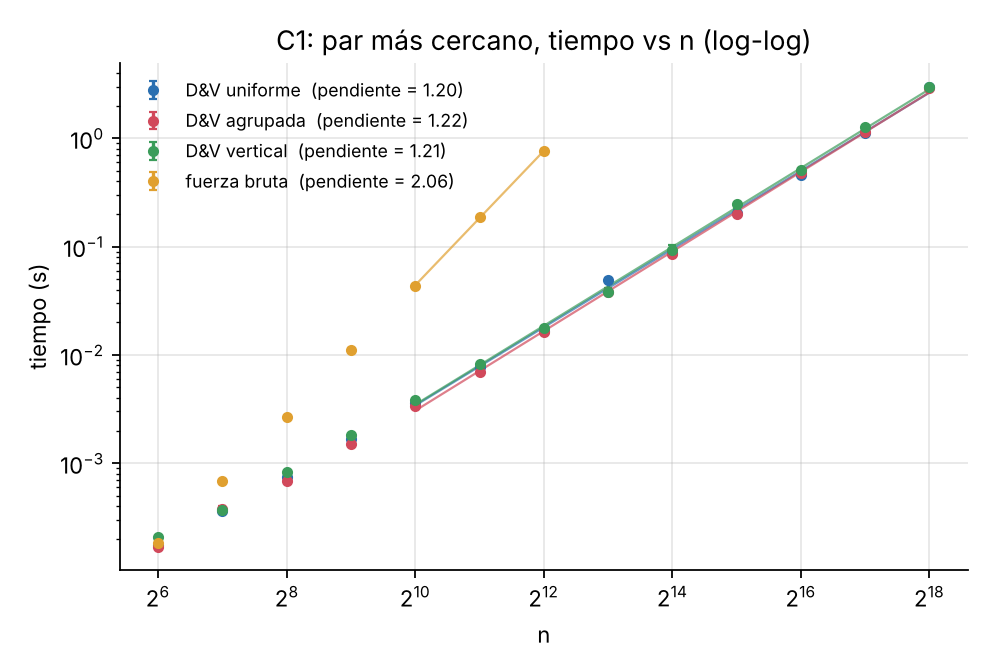
\includegraphics[width=0.49\linewidth]{figuras/c1_loglog.png}\hfill
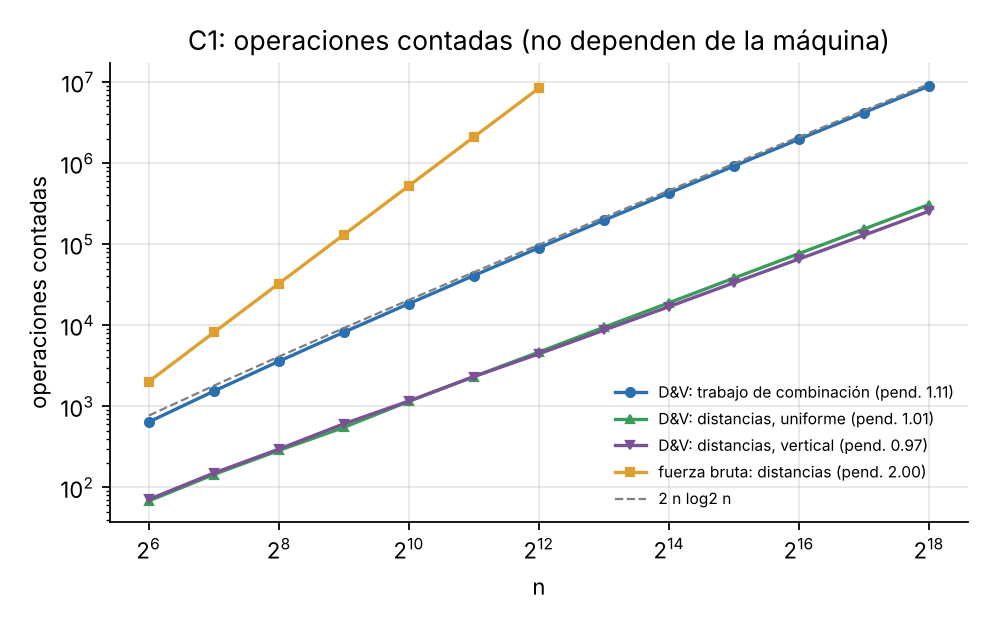
\includegraphics[width=0.49\linewidth]{figuras/c1_operaciones.png}
\caption{C1. Izquierda: tiempo (mediana de 5 repeticiones, barras = rango intercuartílico; pendiente
ajustada en $n\ge2^{10}$). Derecha: operaciones contadas.}
\label{fig:c1}
\end{figure}

\begin{table}[H]
\centering\small
\caption{C1: pendientes medidas frente a las predichas. Para $n\log_2 n$ la pendiente predicha en
$2^{10}..2^{18}$ es $1{,}11$ (no 1).}
\begin{tabular}{lcccc}
\toprule
Serie & Predicha & $2^{10}..2^{14}$ & $2^{14}..2^{18}$ & $2^{10}..2^{18}$ \\
\midrule
D\&V uniforme (tiempo) & $1{,}11$ & $1{,}19$ & $1{,}27$ & $1{,}20$ \\
D\&V agrupada (tiempo) & $1{,}11$ & $1{,}18$ & $1{,}27$ & $1{,}22$ \\
D\&V vertical (tiempo) & $1{,}11$ & $1{,}14$ & $1{,}24$ & $1{,}21$ \\
D\&V trabajo de combinación (conteo) & $1{,}11$ & \multicolumn{3}{c}{$1{,}11$} \\
Fuerza bruta (tiempo, $2^6..2^{12}$) & $2$ & \multicolumn{3}{c}{$2{,}06$} \\
Fuerza bruta (distancias, conteo) & $2$ & \multicolumn{3}{c}{$2{,}00$ \ (exactamente $n(n-1)/2$)} \\
\bottomrule
\end{tabular}
\end{table}

\textbf{Lectura.} (H1.1) Las tres distribuciones dan la misma recta: el algoritmo es $\Th(n\log n)$
aun cuando toda la nube cae en la franja (distribución vertical). La razón $T(n)/(n\log_2 n)$
(figura~\ref{fig:razones}) es casi constante, $\approx0{,}34\,\mu$s, entre $n=2^9$ y $2^{12}$, y
crece de forma suave hasta $0{,}63\,\mu$s en $2^{18}$; ver la discusión (sección~\ref{sec:discusion}).
(H1.2) Fuerza bruta tiene pendiente $2{,}06$. D\&V ya es más rápido desde $n=64$ y en $n=4096$ lo es
$45{,}6$ veces ($0{,}017$\,s frente a $0{,}76$\,s). (H1.3) El máximo de vecinos revisados por punto
de la franja fue 2 (uniforme y agrupada) y 1 (vertical): la cota 7 del Lema~\ref{lem:siete} es de
peor caso y nunca se alcanzó. (H1.4) El trabajo de combinación contado tiene pendiente $1{,}11$,
igual a la de $n\log_2 n$, y la razón combinación$/(n\log_2 n)$ sube de $1{,}67$ a $1{,}89$ acercándose
a 2 (el caso base $n\le3$ ahorra los últimos niveles). Hallazgo: las \emph{distancias} calculadas son
solo $\approx1{,}0$--$1{,}2\,n$ (pendiente $\approx1$): la franja es tan pequeña que el costo
$n\log n$ lo ponen la mezcla y el filtrado, no las distancias.

\begin{figure}[H]
\centering
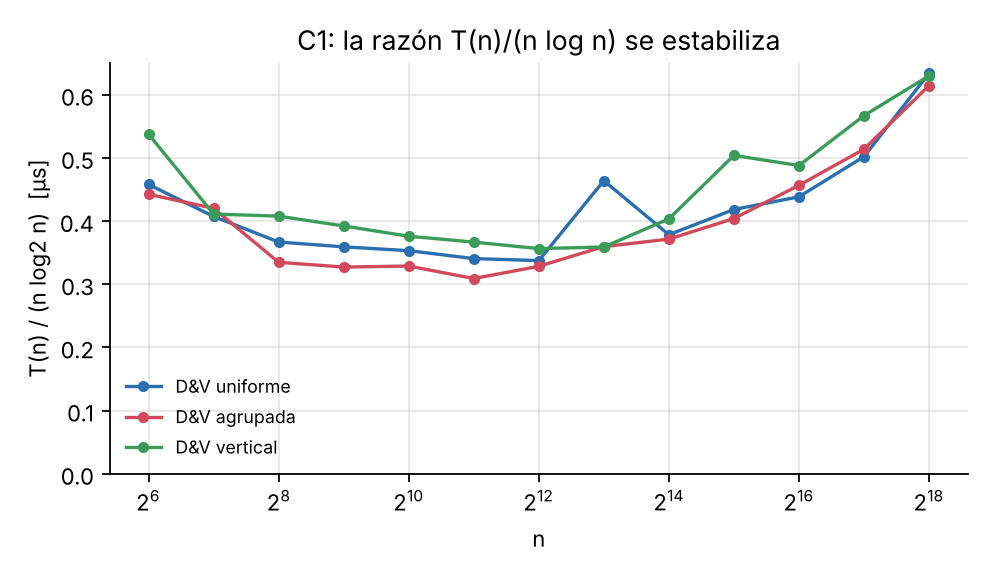
\includegraphics[width=0.6\linewidth]{figuras/c1_razon_nlogn.png}
\caption{C1: $T(n)/(n\log_2 n)$ para las tres distribuciones.}
\label{fig:razones}
\end{figure}

\subsection{C2 -- Mapa de vóxeles}

\begin{figure}[H]
\centering
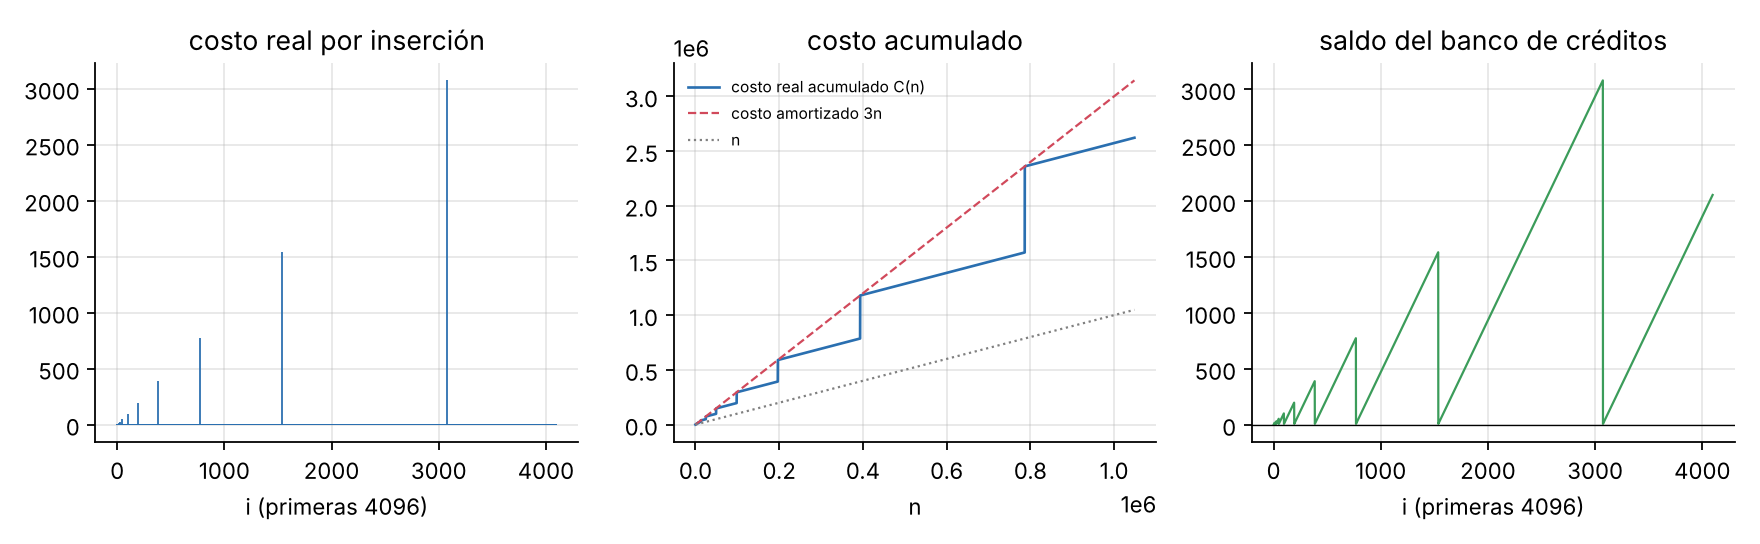
\includegraphics[width=\linewidth]{figuras/c2_metodo_contable.png}
\caption{C2, método contable con $n=2^{20}$ inserciones. Izquierda: picos de costo real en cada
duplicación. Centro: $C(n)$ siempre por debajo de $3n$ (toca la recta justo en cada duplicación).
Derecha: el saldo del banco nunca es negativo.}
\label{fig:c2contable}
\end{figure}

\begin{table}[H]
\centering\small
\caption{C2: método contable y tiempo ($n=2^{20}$ claves distintas).}
\begin{tabular}{lr@{\qquad}lr}
\toprule
Costo real total $C(n)$ & 2\,621\,434 & Duplicaciones & 18 \\
Cota $3n$ & 3\,145\,728 & Capacidad final $m$ & $2^{21}$ \\
$\max_n C(n)/n$ & $2{,}99999$ & Factor de carga final & $0{,}50$ \\
Saldo mínimo del banco & $2$ ($\ge0$) & Pendiente tiempo $2^{10}..2^{20}$ & $1{,}13$ \\
$\min_{n\ge64} C(n)/n$ & $1{,}94$ & Pendiente $2^{10}..2^{14}$ / $2^{14}..2^{20}$ & $1{,}08$ / $1{,}15$ \\
\bottomrule
\end{tabular}
\end{table}

\textbf{Lectura.} (H2.1) Se cumple: $C(n)\le3n$ para todo $n$ y el banco nunca es negativo. La
razón $C(n)/n$ oscila en diente de sierra entre $\approx2$ (justo antes de duplicar) y $3$ (justo
después), tal como predice el análisis. (H2.2) En operaciones el costo por inserción es constante
($\le3$); en tiempo, la pendiente es $1{,}08$ mientras la tabla cabe en caché y $1{,}15$ después:
el tiempo por inserción pasa de $2{,}1\,\mu$s ($n=2^{10}$) a $4{,}7\,\mu$s ($n=2^{20}$) por fallos de
caché, no por el algoritmo (sección~\ref{sec:discusion}).

\begin{figure}[H]
\centering
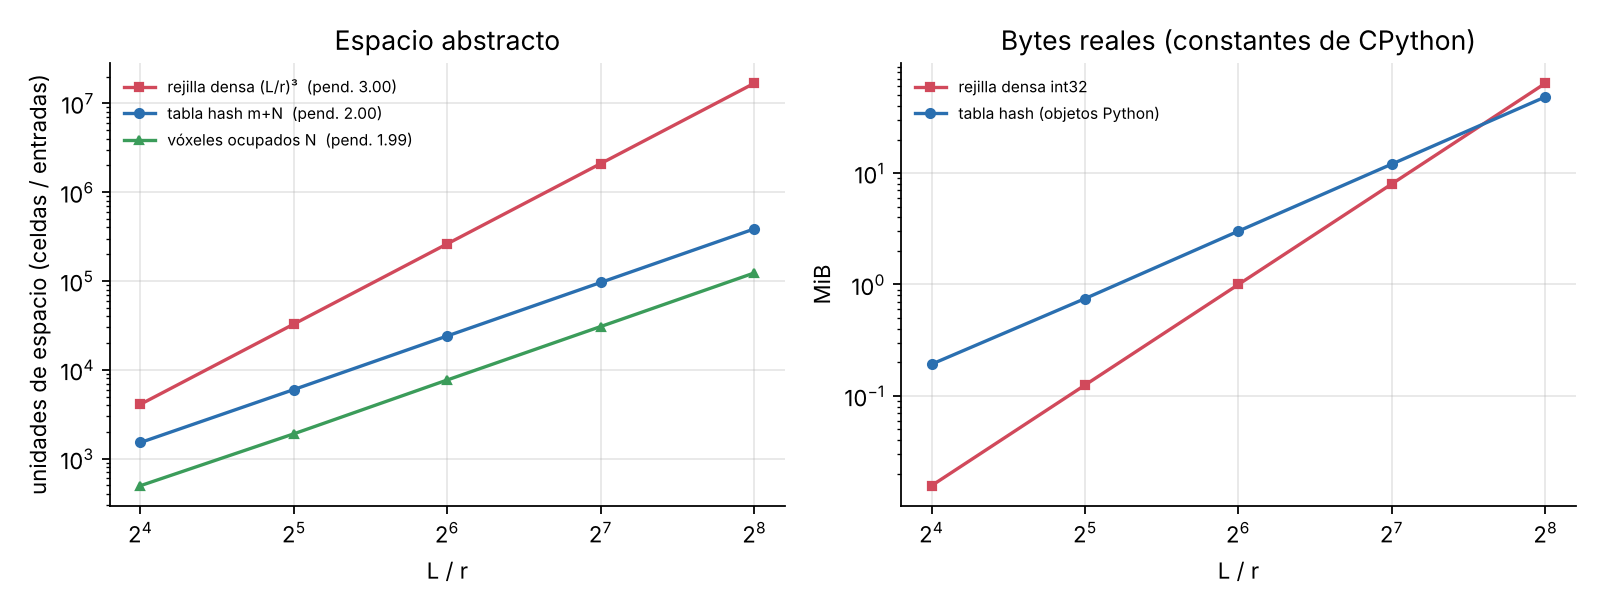
\includegraphics[width=0.92\linewidth]{figuras/c2_espacio.png}
\caption{C2, espacio en una manzana de $L=64$\,m con $r$ de 4\,m a 0,25\,m. Izquierda: unidades
abstractas. Derecha: bytes reales.}
\label{fig:c2esp}
\end{figure}

(H2.3) Respecto a $L/r$, los vóxeles ocupados crecen con pendiente $1{,}99$, la tabla ($m+N$) con
$2{,}00$ y la rejilla densa con $3{,}00$; la tabla frente a $N$ tiene pendiente $1{,}00$ y
$(m+N)/N\approx3{,}1$, dentro del rango teórico $[\tfrac73,\tfrac{11}3]$. En \emph{bytes}, sin
embargo, cada vóxel en la tabla cuesta $\approx410$\,B en CPython (lista, tupla y enteros como objetos)
frente a 4\,B por celda de la rejilla \texttt{int32}: la rejilla gana hasta $L/r=128$ y la tabla
solo pasa a ser más pequeña en $L/r=256$ (48\,MiB frente a 64\,MiB). La ventaja asintótica
$\Th(L/r)$ se confirma, pero la constante de Python mueve el punto de cruce.

\subsection{C3 -- Cobertura mínima}

\begin{table}[H]
\centering\small
\caption{C3: optimalidad en 2000 instancias aleatorias con $n=4..11$ (óptimo por fuerza bruta).}
\begin{tabular}{lr}
\toprule
Instancias factibles / infactibles & 321 / 1679 \\
Voraz ``el que llega más lejos'' igual al óptimo & \textbf{321 de 321 (100\,\%)} \\
Infactibles detectadas por el voraz (excepción \texttt{SinCobertura}) & 1679 de 1679 \\
Voraz ``el más largo primero'' con más tramos que el óptimo & 216 de 321 (67\,\%) \\
Peor caso encontrado para ``el más largo primero'' & 8 tramos frente a 4 óptimos \\
\bottomrule
\end{tabular}
\end{table}

\begin{figure}[H]
\centering
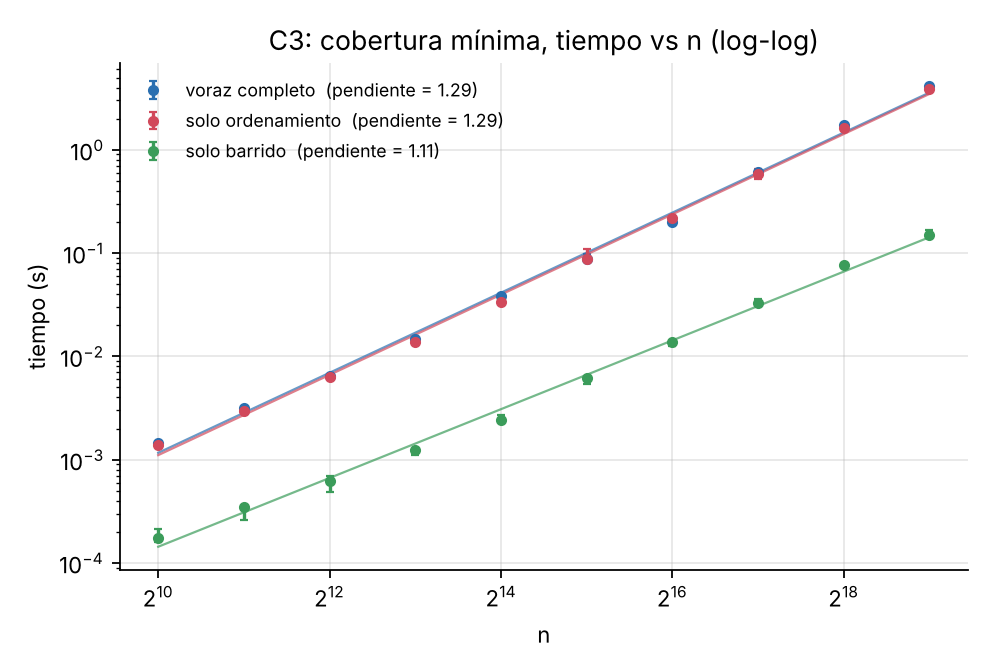
\includegraphics[width=0.49\linewidth]{figuras/c3_loglog.png}\hfill
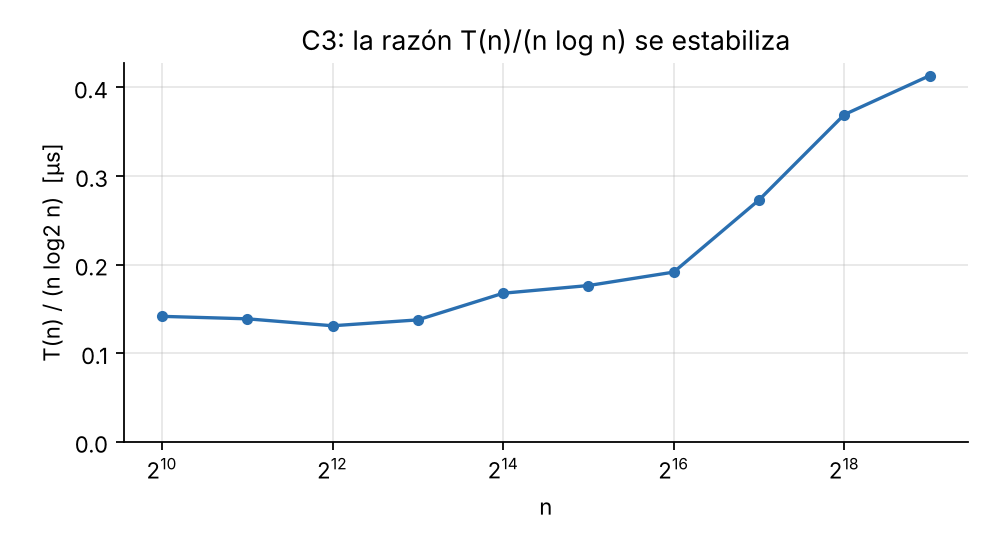
\includegraphics[width=0.49\linewidth]{figuras/c3_razon_nlogn.png}
\caption{C3. Izquierda: tiempo total, del ordenamiento y del barrido. Derecha: $T(n)/(n\log_2 n)$.}
\label{fig:c3}
\end{figure}

\textbf{Lectura.} (H3.1, H3.2) Confirmadas. (H3.3) El tiempo total y el del ordenamiento son casi
idénticos: el merge sort explica $\approx 95$\,\% del tiempo. Pendiente total: $1{,}17$ en
$2^{10}..2^{14}$ (predicha $1{,}10$) y $1{,}38$ en $2^{14}..2^{19}$. Las \emph{comparaciones} contadas
del merge sort tienen pendiente $1{,}11$ y la razón comparaciones$/(n\log_2 n)$ es casi constante
($0{,}88$ a $0{,}93$). $T(n)/(n\log_2 n)$ es constante ($\approx0{,}13\,\mu$s) hasta $n=2^{13}$ y luego
crece. (H3.4) El barrido examina a lo sumo $n$ tramos (verificado en todos los tamaños) y su
pendiente es $0{,}94$ en $2^{10}..2^{14}$ y $1{,}20$ después. La solución usa $\approx 4{,}4$\,\% de los
tramos (por ejemplo, 22\,791 de 524\,288).

% ------------------------------------------------------------- DISCUSIÓN
\section{Discusión}\label{sec:discusion}

\textbf{Dónde coinciden teoría y práctica.} Todo lo que se puede \emph{contar} coincide con la
teoría: $n(n-1)/2$ distancias en fuerza bruta (pendiente $2{,}00$); trabajo de combinación de D\&V y
comparaciones del merge sort con pendiente $1{,}11$, la de $n\log_2 n$; costo contable $C(n)\le3n$
con banco $\ge0$; espacio con pendientes $2$ y $3$; el voraz igual al óptimo en el 100\,\% de los casos.

\textbf{Dónde no coinciden y por qué.} Las pendientes de \emph{tiempo} quedan por encima de lo predicho
cuando $n$ supera $\approx2^{14}$ (C1: $1{,}24$--$1{,}27$; C3: $1{,}38$; C2: $1{,}15$ cuando se esperaba 1).
Tres causas, en orden de importancia:
\begin{enumerate}
  \item \textbf{Jerarquía de memoria.} En CPython cada punto es una tupla con dos objetos
  \texttt{float} ($\approx100$\,B dispersos en el montón). Con $n=2^{14}$ los datos de trabajo ya
  superan los 4\,MiB de caché L2 y cada acceso tiene más probabilidad de fallo. Por eso
  $T(n)/(n\log n)$ es plana mientras los datos caben en caché y luego sube; y por eso las mismas
  operaciones contadas sí dan la pendiente correcta. El modelo RAM supone costo de acceso uniforme;
  el modelo de memoria externa de C5 es justamente el que tiene en cuenta esto.
  \item \textbf{La pendiente de $n\log n$ no es 1.} Es $1+1/\ln n$, unos $1{,}10$--$1{,}12$ en nuestros
  rangos. Comparar contra 1 haría parecer peor el resultado de lo que es.
  \item \textbf{Intérprete y constantes.} El intérprete añade un costo fijo por operación
  ($\approx0{,}3\,\mu$s por unidad de $n\log n$ en C1) y el recolector de basura se desactiva durante la
  medición para no introducir saltos. Las constantes también explican que en bytes la tabla hash solo
  supere a la rejilla densa a partir de $L/r=256$, aunque en unidades abstractas la supera siempre.
\end{enumerate}
La máquina es virtual y compartida (2 núcleos): por eso algunos puntos aislados (C1 uniforme en
$n=2^{13}$) quedan por encima de la recta; usamos la mediana de 5 repeticiones para limitar ese efecto.

% ------------------------------------------------------------- INTEGRIDAD
\section{Integridad y uso de herramientas}

\textbf{Uso de herramientas.} Los algoritmos de C1--C3 están implementados por el
equipo; \texttt{sorted} y \texttt{dict} solo se usan en las pruebas como referencia y NumPy solo para
generar datos y ajustar pendientes. El uso de asistentes de IA se declara en el \texttt{README.md}
del repositorio, como exige la sección 9 del enunciado.

% ------------------------------------------------------------- REFERENCIAS
\section*{Referencias}
\addcontentsline{toc}{section}{Referencias}
\begin{enumerate}[label={[\arabic*]},leftmargin=*]
\small
\item T. H. Cormen, C. E. Leiserson, R. L. Rivest y C. Stein. \emph{Introduction to Algorithms}, 4.ª ed.
MIT Press, 2022. (Teorema Maestro, cap.~4; análisis amortizado, cap.~16; tablas hash, cap.~11;
par más cercano, sec.~33.4.)
\item J. Kleinberg y É. Tardos. \emph{Algorithm Design}. Pearson, 2006. (Algoritmos voraces:
argumentos de intercambio y ``el voraz se mantiene adelante'', cap.~4; par más cercano, sec.~5.4.)
\item M. I. Shamos y D. Hoey. Closest-point problems. En \emph{16th Annual Symposium on Foundations of
Computer Science}, pp.~151--162, IEEE, 1975.
\item M. Ben-Or. Lower bounds for algebraic computation trees. En \emph{Proc.\ 15th ACM Symposium on
Theory of Computing}, pp.~80--86, 1983.
\item M. Teschner, B. Heidelberger, M. Müller, D. Pomerantes y M. Gross. Optimized spatial hashing
for collision detection of deformable objects. En \emph{Vision, Modeling, and Visualization}, 2003.
\item M. Nießner, M. Zollhöfer, S. Izadi y M. Stamminger. Real-time 3D reconstruction at scale using
voxel hashing. \emph{ACM Transactions on Graphics}, 32(6), 2013.
\item A. Aggarwal y J. S. Vitter. The input/output complexity of sorting and related problems.
\emph{Communications of the ACM}, 31(9):1116--1127, 1988. (Modelo de memoria externa, para C5.)
\end{enumerate}

% ------------------------------------------------------------- ANEXO: CÓDIGO
\clearpage
\appendix
\section{Código de C1, C2 y C3 con pruebas}\label{anexo:codigo}

Código fuente completo de los componentes del avance, tal como está en el repositorio. Cada
componente tiene su carpeta con la implementación y su archivo de pruebas \texttt{test\_*.py}
(pytest). Se incluyen también el merge sort propio (lo usan C1 y C3, porque el núcleo no puede usar
\texttt{sorted}), el protocolo de medición y el generador de datos. Para ejecutar las pruebas desde la
raíz del repositorio: \texttt{python -m pytest -v}. La salida está en la sección~\ref{anexo:pytest}.

\subsection{Utilidades comunes}
\codigo{comun/ordenamiento.py}{Merge sort propio, estable, $\Theta(n\log n)$.}
\codigo{comun/test_ordenamiento.py}{Pruebas del merge sort.}
\codigo{comun/medicion.py}{Protocolo de medición (sección 4.3 del enunciado).}

\subsection{Generador de datos (semilla fija = 6)}
\codigo{datos/generador.py}{Nubes de puntos 2D y 3D y tramos de sensado.}
\codigo{datos/test_generador.py}{Pruebas del generador.}

\subsection{C1 -- Par de puntos más cercanos (divide y vencerás)}
\codigo{c1_par_mas_cercano/par_cercano.py}{Divide y vencerás $\Theta(n\log n)$ y fuerza bruta $\Theta(n^2)$.}
\codigo{c1_par_mas_cercano/test_par_cercano.py}{Pruebas de C1.}

\subsection{C2 -- Mapa de vóxeles como tabla hash dinámica}
\codigo{c2_mapa_voxeles/tabla_hash.py}{Tabla hash con duplicación e instrumentación del método contable.}
\codigo{c2_mapa_voxeles/mapa_voxeles.py}{Voxelización y comparación de espacio con la rejilla densa.}
\codigo{c2_mapa_voxeles/test_tabla_hash.py}{Pruebas de C2.}

\subsection{C3 -- Voraz: cobertura mínima de un segmento con intervalos}
\codigo{c3_cobertura_intervalos/cobertura.py}{Voraz, verificador, fuerza bruta y regla alternativa (contraejemplo).}
\codigo{c3_cobertura_intervalos/test_cobertura.py}{Pruebas de C3.}

\subsection{Configuración y ejecución de las pruebas}\label{anexo:pytest}
\par\smallskip\noindent{\small\bfseries\texttt{pytest.ini}}\enspace{\small\color{gris}Configuración de pytest.}
\lstinputlisting[style=salida]{codigo/pytest.ini}
\par\smallskip\noindent{\small\bfseries Salida de \texttt{python -m pytest -v}}\enspace{\small\color{gris}23 pruebas aprobadas.}
\lstinputlisting[style=salida]{codigo/salida_pytest.txt}

\end{document}
